\documentclass[aspectratio=169,11pt]{beamer}

% ---------------- Theme and colours ----------------
\usetheme{Madrid}
\usecolortheme{default}
\definecolor{qblue}{RGB}{51,51,170}
\definecolor{qlight}{RGB}{232,236,250}
\definecolor{qgreen}{RGB}{27,140,90}
\definecolor{qred}{RGB}{190,50,50}
\definecolor{qgray}{RGB}{90,90,90}
\setbeamercolor{structure}{fg=qblue}
\setbeamercolor{palette primary}{bg=qblue,fg=white}
\setbeamercolor{palette secondary}{bg=qblue!80!black,fg=white}
\setbeamercolor{palette tertiary}{bg=qblue!60!black,fg=white}
\setbeamercolor{frametitle}{bg=qblue,fg=white}
\setbeamercolor{block title}{bg=qblue,fg=white}
\setbeamercolor{block body}{bg=qlight}
\setbeamercolor{block title alerted}{bg=qred,fg=white}
\setbeamercolor{block body alerted}{bg=qred!8}
\setbeamercolor{block title example}{bg=qgreen,fg=white}
\setbeamercolor{block body example}{bg=qgreen!8}
\setbeamertemplate{navigation symbols}{}
\setbeamertemplate{itemize items}[circle]

\usepackage{booktabs}
\usepackage{array}
\usepackage{appendixnumberbeamer}
\usepackage{textcomp}
\usepackage{tikz}
\usetikzlibrary{arrows.meta,positioning,shapes.geometric}
\graphicspath{{figures/}}

\newcommand{\good}[1]{\textcolor{qgreen}{\textbf{#1}}}
\newcommand{\bad}[1]{\textcolor{qred}{\textbf{#1}}}

\title[Adaptive QEM for Non-Stationary Noise]{Transformer-Based Real-Time Adaptive Quantum Error Mitigation for Non-Stationary Noise}
\subtitle{Final Review}
\author[Hasini, Saanvika, Dharshini]{Madhu Hasini (CB.AI.U4AID24060) \and Saanvika (CB.AI.U4AID24047) \and Dharshini (CB.AI.U4AID24013)}
\institute[]{[Department, Institution]}
\date{October 2026}

\begin{document}

% =========================================================== 1
\begin{frame}
\titlepage
\end{frame}

% =========================================================== 2
\begin{frame}{Outline}
\begin{columns}[T]
\column{0.48\textwidth}
\begin{enumerate}
\item Motivation and problem
\item Base paper and research gaps
\item Our contributions
\item Dataset and leakage-safe splits
\item Forecasting calibration drift
\item Noise model and mitigation actions
\end{enumerate}
\column{0.48\textwidth}
\begin{enumerate}
\setcounter{enumi}{6}
\item Adaptive policies and fair comparison
\item Results: hypothesis tests, all policies
\item Why forecasting and the bandit fell short
\item Robustness and an exploratory model
\item Conclusion, limitations, future work
\item Backup slides
\end{enumerate}
\end{columns}
\end{frame}

% =========================================================== 3
\begin{frame}{Motivation: quantum noise is not constant}
\begin{columns}[T]
\column{0.5\textwidth}
\begin{itemize}
\item Today's qubits are noisy: relaxation ($T_1$), dephasing ($T_2$), gate errors and readout errors bias every measured result.
\item \textbf{Quantum error mitigation (QEM)} recovers better estimates by post-processing several related runs.
\item Its settings (ZNE scale factors, extrapolator, twirling) are usually \textbf{fixed in advance}.
\item But the hardware \textbf{drifts}: IBM recalibrates every day and the values change, sometimes abruptly.
\end{itemize}
\column{0.5\textwidth}
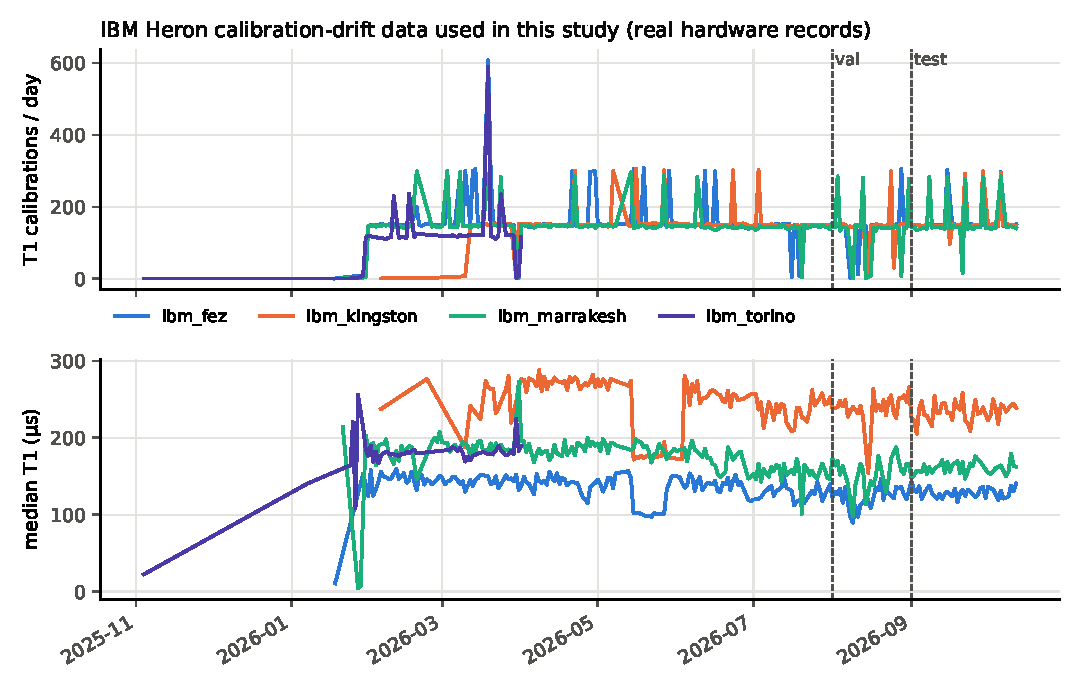
\includegraphics[width=\linewidth]{data_coverage.pdf}
{\scriptsize Real IBM data used in this project: calibrations per day (top) and median $T_1$ per device (bottom). Note the drop on two devices in mid-May 2026.}
\end{columns}
\end{frame}

% =========================================================== 4
\begin{frame}{Problem statement and research question}
\begin{block}{Problem}
A mitigation setting chosen for yesterday's noise can be a poor choice for today's. Can we choose QEM settings that fit the noise that will be present when the circuit actually runs?
\end{block}
\vspace{0.3cm}
\begin{block}{Research question}
Can Transformer-based forecasting of real calibration drift improve QEM decisions compared with
\begin{itemize}
\item a \textbf{fixed} mitigation configuration,
\item adapting to the \textbf{latest published calibration} (persistence), and
\item a \textbf{contextual-bandit} adaptive ZNE (our base paper),
\end{itemize}
under the same shot budget?
\end{block}
\end{frame}

% =========================================================== 5
\begin{frame}{Base paper and research gaps}
\footnotesize
\begin{columns}[T]
\column{0.48\textwidth}
\begin{block}{Base paper}
R.~Rahman and D.~C.~Nguyen, ``Quantum Noise Mitigation With Adaptive Zero-Noise Extrapolation: A Contextual Multi-Armed Bandits Approach'', \textit{IEEE JSAC}, vol.~44, pp.~5600--5614, 2026.
\begin{itemize}
\item LinUCB bandit picks the ZNE folding set online
\item In their simulations (variational classifiers, prescribed drift): about 39--41\% fewer circuit round trips than fixed \{1,3,5\} folding
\item We compare with \textbf{our reimplementation} of their bandit (extended action space; results apply to this implementation, not to the method in general)
\end{itemize}
\end{block}
\column{0.48\textwidth}
\begin{alertblock}{Gaps we identified}
\begin{itemize}
\item \textbf{Reactive}, no forecast of future noise
\item \textbf{Synthetic} drift profile, not real calibrations
\item Only the folding set is adapted
\item A bandit needs a \textbf{reward}; for expectation values the ideal answer is unknown
\item Learned models rarely compared with \textbf{simple baselines}
\end{itemize}
\end{alertblock}
\end{columns}
\end{frame}

% =========================================================== 6
\begin{frame}{Our contributions}
\begin{enumerate}
\item \textbf{Benchmark on real drift:} 101,891 calibration states from 600 qubits on 4 IBM Heron processors, linked to adaptive ZNE and Pauli-twirling decisions, with leakage-safe chronological, unseen-qubit and unseen-device tests.
\vspace{0.25cm}
\item \textbf{Calibration-informed adaptive controller:} jointly selects ZNE scale factors, extrapolator and twirling. In simulation:
\begin{itemize}
\item \good{$-4.2$\% to $-5.6$\%} error vs best fixed configuration
\item \good{$-15$\% to $-19$\%} error vs our reimplementation of the base paper's bandit, same shot budget
\end{itemize}
\vspace{0.25cm}
\item \textbf{Pre-registered test of Transformer forecasting:} better forecasts did \bad{not} give better decisions; a value-of-information analysis bounds the possible gain at 1.4--7.1\%, concentrated in abrupt device changes.
\end{enumerate}
\end{frame}

% =========================================================== 7
\begin{frame}{Dataset: real IBM calibration drift}
\begin{columns}[T]
\column{0.5\textwidth}
\begin{table}
\small
\begin{tabular}{lr}
\toprule
Rows in dataset file & 16,140,252 \\
Genuine measurements & 2,024,027 \\
Calibration states used$^{*}$ & 101,891 \\
Backends & 4 (IBM Heron) \\
Qubits & 600 \\
Period & Jan--Oct 2026 \\
Calibration spacing & 24.8 h (median) \\
\bottomrule
\end{tabular}
\end{table}
{\scriptsize $^{*}$One assembled record per qubit and $T_1$ calibration. Source: Hugging Face \texttt{phanerozoic/qiskit-calibration-drift}, revision pinned, CC-BY-4.0.}
\column{0.5\textwidth}
\textbf{Properties per qubit state}
\begin{itemize}
\item $T_1$, $T_2$ (\textmu s)
\item single-qubit (sx) gate error
\item readout errors
\item CZ error of each coupled pair
\item calibration age, time gaps
\end{itemize}
\textbf{Compared with the first version}
\begin{itemize}
\item 1,000 rows, 10 qubits $\rightarrow$ 101,891 states, 600 qubits
\item $T_1$ only $\rightarrow$ five properties
\end{itemize}
\end{columns}
\end{frame}

% =========================================================== 8
\begin{frame}{Data cleaning and leakage-safe splits}
\begin{columns}[T]
\column{0.5\textwidth}
\textbf{Cleaning}
\begin{itemize}
\item $T_1$/$T_2$ stored in \textbf{seconds before} and \textbf{microseconds after} a May 2026 schema change $\rightarrow$ converted (this bug had broken the first pipeline)
\item Only \textbf{genuine} measurements kept: value changed (a heuristic; the data have no new-measurement flag). 89\% of gate-error events were re-timestamps
\item Failure ceilings ($\geq 0.999$) removed
\item Every value joined by its \textbf{publication time}, so no future information leaks in
\end{itemize}
\column{0.5\textwidth}
\textbf{Splits}
\begin{itemize}
\item \textbf{Chronological}: train $<$ 1 Aug, validation Aug, test 1 Sep -- 12 Oct 2026
\item \textbf{Unseen qubits}: 20\% of qubits never used for training
\item \textbf{Unseen device}: ibm\_marrakesh held out completely
\item Unseen qubits and device are scored on the \textbf{test period} only
\item Hyperparameters chosen on validation only; test evaluated \textbf{once}, after freezing all inputs
\end{itemize}
\end{columns}
\end{frame}

% =========================================================== 9
\begin{frame}{End-to-end pipeline}
\centering
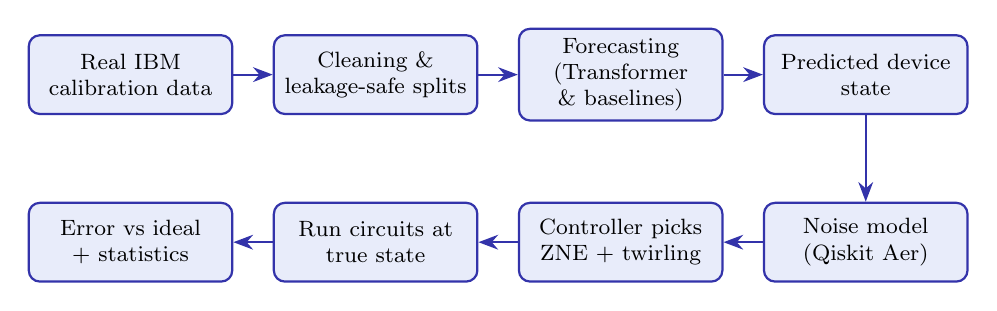
\begin{tikzpicture}[node distance=0.45cm and 0.5cm,
  box/.style={rectangle, rounded corners, draw=qblue, fill=qlight, thick, align=center, minimum height=1.0cm, text width=2.35cm, font=\footnotesize},
  arr/.style={-{Stealth[length=2.5mm]}, thick, qblue}]
\node[box] (a) {Real IBM\\calibration data};
\node[box, right=of a] (b) {Cleaning \&\\leakage-safe splits};
\node[box, right=of b] (c) {Forecasting\\(Transformer \& baselines)};
\node[box, right=of c] (d) {Predicted device\\state};
\node[box, below=1.1cm of d] (e) {Noise model\\(Qiskit Aer)};
\node[box, left=of e] (f) {Controller picks\\ZNE + twirling};
\node[box, left=of f] (g) {Run circuits at\\true state};
\node[box, left=of g] (h) {Error vs ideal\\+ statistics};
\draw[arr] (a) -- (b); \draw[arr] (b) -- (c); \draw[arr] (c) -- (d);
\draw[arr] (d) -- (e); \draw[arr] (e) -- (f); \draw[arr] (f) -- (g); \draw[arr] (g) -- (h);
\end{tikzpicture}
\vspace{0.3cm}

\small The same controller is fed different state estimates: latest calibration (persistence), window mean, ridge, Transformer, or the true state (oracle). Only the estimate changes, so differences come from the forecasts.
\end{frame}

% =========================================================== 10
\begin{frame}{Result 1: forecasting skill relative to persistence (test)}
\begin{columns}[c]
\column{0.62\textwidth}
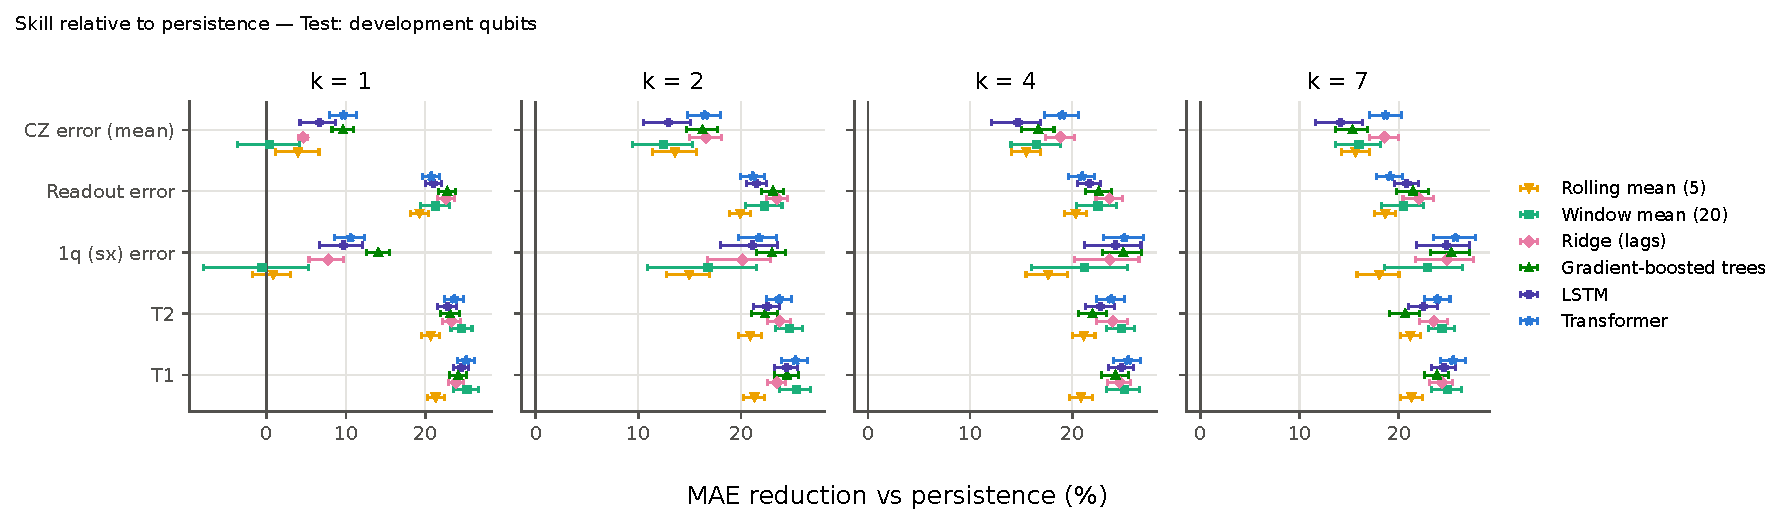
\includegraphics[width=\linewidth]{skill_vs_persistence_test_primary.pdf}
\column{0.38\textwidth}
\begin{itemize}\small
\item Bars to the right of zero = better than persistence.
\item Models: persistence, window means, ridge, trees, LSTM, Transformer (details in backup).
\item The Transformer beats persistence by \good{9.7--25.7\%} (all learned models: 4.6--25.7\%).
\item The Transformer never beats \textbf{every} baseline: readout error is better with ridge; $T_1$, $T_2$ with a simple window mean.
\item \bad{H1 not supported} (0 of 15 pre-registered cells).
\end{itemize}
\end{columns}
\end{frame}

% =========================================================== 11
\begin{frame}{Quantum backend: noise model and circuits}
\footnotesize
\begin{columns}[T]
\column{0.5\textwidth}
\textbf{Noise model per chain and day}
\begin{itemize}
\item Chains of 4 coupled qubits from the real coupling map
\item Relaxation from $T_1$, $T_2$ over real gate times (sx 24--36 ns, CZ 68 ns)
\item Depolarising error fills only the gap left by relaxation, so the total matches IBM's reported error (within 0.07\%); no double counting
\item Readout and idle errors \textbf{not simulated}
\item Optional coherent CZ phase error, 0.03 rad
\item Execution simulated with Qiskit Aer (density matrix)
\end{itemize}
\column{0.5\textwidth}
\textbf{Benchmark circuits} (native CZ, sx, rz, x)
\begin{table}\scriptsize
\begin{tabular}{lcc}
\toprule
Circuit & Depths & CZ gates \\
\midrule
Hardware-efficient ansatz & 4, 8 & 12, 24 \\
Trotterised TFIM & 3, 6 & 18, 36 \\
QAOA (path graph) & 2, 4 & 12, 24 \\
\bottomrule
\end{tabular}
\end{table}
Observables: Z and X Pauli strings with $|\langle P\rangle| > 0.2$; ideal values known exactly.
\end{columns}
\end{frame}

% =========================================================== 12
\begin{frame}{Mitigation actions: ZNE and Pauli twirling}
\footnotesize
\begin{columns}[T]
\column{0.5\textwidth}
\begin{block}{Zero-noise extrapolation}
\begin{itemize}
\item Amplify noise by folding each CZ: CZ $\rightarrow$ CZ (CZ CZ)$^n$
\item Scale sets \{1,3\}, \{1,2,3\}, \{1,3,5\}, \{1,3,5,7\}
\item Fits: linear, Richardson, exponential, quadratic; fits use the \textbf{achieved} scale
\item Exponential falls back to linear if values change sign; estimates clipped to $[-1,1]$
\end{itemize}
\end{block}
\column{0.5\textwidth}
\begin{block}{Pauli twirling}
\begin{itemize}
\item 8 frames per circuit, drawn uniformly from the 16 Pauli pairs that leave CZ unchanged (fixed seed)
\item Turns coherent errors into stochastic Pauli errors
\item Folded and twirled circuits reproduce the ideal values exactly without noise (tested)
\item Shots are split over frames: more circuits, \textbf{same shots}
\end{itemize}
\end{block}
\end{columns}
\vspace{0.1cm}
\begin{exampleblock}{Shared action set}
14 actions = no mitigation, twirling only, and 6 ZNE settings with and without twirling. Every policy uses the \textbf{same 8,192 shots per observable}.
\end{exampleblock}
\end{frame}

% =========================================================== 13
\begin{frame}{Adaptive policies and a fair comparison}
\begin{table}\small
\begin{tabular}{>{\raggedright\arraybackslash}p{3.4cm}>{\raggedright\arraybackslash}p{9.2cm}}
\toprule
\textbf{Policy} & \textbf{How it chooses the action} \\
\midrule
No mitigation & Raw circuit only \\
Best fixed & One action, chosen on validation data (protocol text said training; deviation disclosed) \\
Persistence & Controller simulates all actions on the \textbf{latest calibration}, picks the lowest predicted error \\
Window mean / Ridge / \textbf{Transformer} & Same controller, fed the \textbf{forecast} state for execution time \\
Contextual bandit (base paper) & \textbf{Our reimplementation} of their LinUCB; Clifford-probe reward from 1,024 of the 8,192 shots, main estimate 7,168; feedback after execution \\
Oracle (reference only) & Controller fed the \textbf{true} execution state \\
\bottomrule
\end{tabular}
\end{table}
\small Same 14 actions, same total shot budget and test conditions for all. Information differs by design: model-based policies use calibration estimates, the bandit uses probe feedback. Our bandit uses the extended 14-action space (the paper used 3 folding sets) and a probe reward instead of a classification loss; it is tuned on validation and learns online for two months before testing.
\end{frame}

% =========================================================== 14
\begin{frame}{Result 2: hypothesis tests (test period)}
\begin{table}\small
\begin{tabular}{lll}
\toprule
\textbf{Hypothesis} & \textbf{Result (95\% CI)} & \textbf{Verdict} \\
\midrule
H1 forecasting & Transformer never beats all baselines & \bad{Not supported} \\
H2 vs persistence, 1 day & $+0.02\%$ \; [$-0.29$, $+0.54$] & \bad{Not supported} \\
H2 at 4 / 7 days & $-0.41\%$ / $-0.05\%$, not significant & \bad{Not supported} \\
H3 vs best fixed & $-5.6\%$ (1 d), $-4.2\%$ (4 d), $-0.3\%$ (7 d) & \good{Supported (1, 4 d)} \\
H3 stationary noise & $-4.9\%$ \; [$-7.4$, $-1.0$] & \good{Supported} \\
H4 vs bandit & $-15.0\%$ / $-18.7\%$ / $-14.5\%$ & \good{Supported} \\
\bottomrule
\end{tabular}
\end{table}
{\scriptsize Percentages: difference in mean error $\div$ the comparator's error. R1 and R2 pooled (per protocol); e.g.\ vs best fixed at 1 day: R1 $-2.9$\%, R2 $-8.2$\%, pooled $-5.6$\%. 1 day: 8,028 decision units from 29 chains.}
\begin{exampleblock}{In one line}
In our simulated benchmark, adapting to the calibration helps; forecasting the calibration does not add to it.
\end{exampleblock}
\end{frame}

% =========================================================== 15
\begin{frame}{Result 2 (cont.): all policies on one scale}
\begin{table}\scriptsize
\begin{tabular}{lccccc}
\toprule
\textbf{Policy} & \textbf{Error} & \textbf{vs persistence (\%)} & \textbf{95\% CI} & \textbf{Holm $p$} & \textbf{Shots/obs.} \\
\midrule
Latest calibration (persistence) & 0.0238 & -- & -- & -- & 8,192 \\
No mitigation & 0.0462 & $+94.4$ & [$+64.1$, $+132.8$] & $<$0.01 & 8,192 \\
Best fixed (global) & 0.0252 & $+6.0$ & [$+1.9$, $+12.6$] & $<$0.01 & 8,192 \\
Best fixed (per circuit) & 0.0248 & $+4.3$ & [$+0.1$, $+11.0$] & 0.14 & 8,192 \\
Bandit, probe reward & 0.0280 & $+17.7$ & [$+14.9$, $+21.5$] & $<$0.01 & 7,168 + 1,024 \\
Bandit, warm start & 0.0267 & $+12.2$ & [$+8.7$, $+16.7$] & $<$0.01 & 7,168 + 1,024 \\
Window-mean forecast & 0.0241 & $+1.1$ & [$-0.5$, $+4.0$] & 1.00 & 8,192 \\
Ridge forecast & 0.0238 & $+0.1$ & [$-0.2$, $+0.5$] & 1.00 & 8,192 \\
Transformer forecast & 0.0238 & $+0.0$ & [$-0.3$, $+0.5$] & 1.00 & 8,192 \\
True state (oracle)$^{\dagger}$ & 0.0234 & $-1.6$ & [$-2.8$, $-0.7$] & $<$0.01 & 8,192 \\
\bottomrule
\end{tabular}
\end{table}
{\scriptsize Test set, 1 day ahead, development chains, R1 + R2; 8,028 units, 29 chains. (policy $-$ persistence) $\div$ persistence; positive = worse. Two-sided $p$, Holm-adjusted over 9 comparisons. Descriptive summary computed after the pre-registered tests. $^{\dagger}$Not realisable.}
\end{frame}

% =========================================================== 16
\begin{frame}{Why forecasting did not help: value of information}
\begin{columns}[T]
\column{0.5\textwidth}
\textbf{Oracle gain over persistence} (perfect forecast)
\begin{itemize}
\item 1 day: \textbf{1.4--1.7\%}
\item 4 days: \textbf{3.0--3.7\%}
\item 7 days: \textbf{5.2--7.1\%}
\end{itemize}
\vspace{0.2cm}
\textbf{Where is the gain?} Decisions with the largest CZ change (top quarter, $\approx 2.3\times$):
\begin{itemize}
\item oracle beats persistence by \textbf{6.4 / 9.3 / 14.1\%}
\item persistence is then \bad{worse} than the best fixed action
\end{itemize}
\column{0.5\textwidth}
\begin{alertblock}{Forecast accuracy $\neq$ decision value}
\begin{itemize}
\item In those large-change cases the Transformer forecast is closer than persistence 90--97\% of the time...
\item ...but recovers only $\approx$1.2--1.4\% of the possible 6--14\%.
\item Forecasts gain accuracy by pulling values toward the average; that rarely changes which mitigation action is best.
\end{itemize}
\end{alertblock}
\end{columns}
\end{frame}

% =========================================================== 17
\begin{frame}{Why the bandit underperformed}
\begin{columns}[c]
\column{0.55\textwidth}
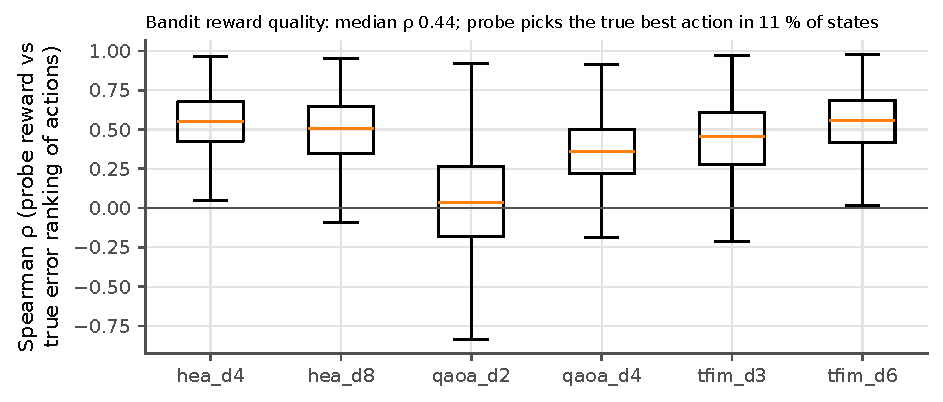
\includegraphics[width=\linewidth]{probe_reward_quality.pdf}
\column{0.45\textwidth}
\begin{itemize}\small
\item The bandit's reward is the error on a \textbf{Clifford probe} circuit (ideal value known).
\item The plot shows how well that reward ranks the 14 actions compared with the true error: median correlation \textbf{0.03--0.56}.
\item The probe finds the truly best action in only \bad{6--14\%} of cases, and costs 12.5\% of the shots.
\item Even with the true error as reward, our bandit implementation only matched a fixed action per circuit.
\end{itemize}
\end{columns}
\end{frame}

% =========================================================== 18
\begin{frame}{Robustness checks (pre-registered, test period)}
\begin{table}\small
\begin{tabular}{lccc}
\toprule
\textbf{Transformer-driven adaptation vs} & \textbf{Main study} & \textbf{8 new circuits} & \textbf{6-qubit chains} \\
\midrule
Persistence & $+0.02\%$ & $-0.42\%$ & $-0.35\%$ \\
Best fixed & \good{$-5.6\%$} & \good{$-5.7\%$} & $-3.6\%$ \\
Bandit & \good{$-15.0\%$} & \good{$-17.8\%$} & -- \\
Oracle gap (ceiling) & 1.4--1.7\% & 2.5\% & 2.6\% \\
\bottomrule
\end{tabular}
\end{table}
\begin{itemize}
\item Same conclusions for new random circuit instances and for larger (6-qubit) chains.
\item Green = 95\% confidence interval excludes zero. Percentages are relative to the comparator's error.
\end{itemize}
\end{frame}

% =========================================================== 19
\begin{frame}{Exploratory: a decision-focused Transformer}
\begin{columns}[T]
\column{0.5\textwidth}
\textbf{Idea}
\begin{itemize}
\item Let the Transformer read the chain's history and \textbf{directly correct} the predicted error of each action
\item Trained on simulated outcomes; judged on validation only
\end{itemize}
\textbf{Result (1 day ahead)}
\begin{itemize}
\item vs persistence: \bad{$+0.28\%$} (worse)
\item 4 / 7 days: $-0.05\%$ / $-0.14\%$, not significant
\end{itemize}
\column{0.5\textwidth}
\begin{alertblock}{Check for artifacts}
A control model \textbf{without any history} did slightly better ($-0.22\%$). This is consistent with learning a simulator-specific correction; the experiment does not show that the model learned decision-relevant drift. Adding history made things worse.
\end{alertblock}
\vspace{0.2cm}
Did not meet its pre-registered criterion. Evaluated on \textbf{validation data only}, never on an independent test period; reported as exploratory work.
\end{columns}
\end{frame}

% =========================================================== 20
\begin{frame}{Conclusion}
\begin{exampleblock}{Three separate findings (simulated execution, real IBM calibration drift)}
\begin{enumerate}
\item \textbf{Calibration-informed adaptation improved the tested benchmark} under the evaluated conditions: $-4$ to $-6$\% error vs the best fixed setting and $-15$ to $-19$\% vs our reimplementation of the base paper's bandit, with no extra shots.
\item \textbf{Transformer forecasting gave no statistically reliable improvement} over the latest calibration at 1, 4 or 7 days (nor did ridge or window-mean forecasts).
\item \textbf{The decision-focused Transformer did not pass} its validation criterion (exploratory).
\end{enumerate}
\end{exampleblock}
\begin{block}{Answer to the research question}
Forecasting calibration drift added no demonstrated decision value beyond using the latest calibration; a perfect forecast would be worth only 1.4--7.1\%, mostly during abrupt device changes.
\end{block}
\end{frame}

% =========================================================== 21
\begin{frame}{Limitations and future work}
\begin{columns}[T]
\column{0.5\textwidth}
\begin{alertblock}{Limitations}
\begin{itemize}
\item Execution simulated, not run on hardware
\item Readout and idle errors not modelled
\item 4- and 6-qubit chains
\item Next published calibration used as the true state
\item Controller needs an accurate noise model
\end{itemize}
\end{alertblock}
\column{0.5\textwidth}
\begin{block}{Future work}
\begin{itemize}
\item Train forecasters for decision quality, not accuracy
\item Use forecasts only when a large change is predicted
\item Test on newer, unseen calibration data
\item Validate on IBM hardware
\item Larger circuits with cheaper surrogate controllers
\end{itemize}
\end{block}
\end{columns}
\end{frame}

% =========================================================== 22
\begin{frame}
\centering
\vspace{1.5cm}
{\Huge \textcolor{qblue}{Thank you}}\\[0.6cm]
{\Large Questions?}\\[1.0cm]
{\small Code, data provenance and results: \texttt{python3 reproduce.py all}.\\ The confirmatory pipeline was rerun from scratch on 13 Oct 2026; all key result files were byte-identical.}
\end{frame}

\appendix
% =========================================================== Backup
\begin{frame}
\centering
\vspace{2cm}
{\LARGE \textcolor{qblue}{Backup slides}}\\[0.5cm]
{\small Forecasting details, evaluation protocol, additional result plots}
\end{frame}

% =========================================================== B1
\begin{frame}{Forecasting calibration drift: models}
\small
\begin{columns}[T]
\column{0.5\textwidth}
\textbf{Task}
\begin{itemize}
\item Input: last 20 calibrations of a qubit (19 features)
\item Output: change in log $T_1$, $T_2$, sx error, readout error, CZ error
\item Horizons: 1, 2, 4 and 7 \textbf{calibration cycles} ahead (median spacing 24.8 h, so not exactly days)
\item Test: 9,745 forecasts from 247 qubits at $k=1$
\end{itemize}
\textbf{Metric}
\begin{itemize}
\item MAE of the log value ($\approx$ relative error), each qubit weighted equally
\item 95\% cluster-bootstrap confidence intervals
\end{itemize}
\column{0.5\textwidth}
\textbf{Models compared}
\begin{itemize}
\item Persistence (latest value)
\item Rolling mean (5) and window mean (20)
\item Ridge regression, gradient-boosted trees
\item LSTM
\item \textbf{Transformer}: positional encoding, multi-horizon head, 5-seed ensemble (1 layer, width 32, 4 heads)
\end{itemize}
\end{columns}
\end{frame}

% =========================================================== B2
\begin{frame}{Result 1: forecast error vs horizon (test)}
\centering
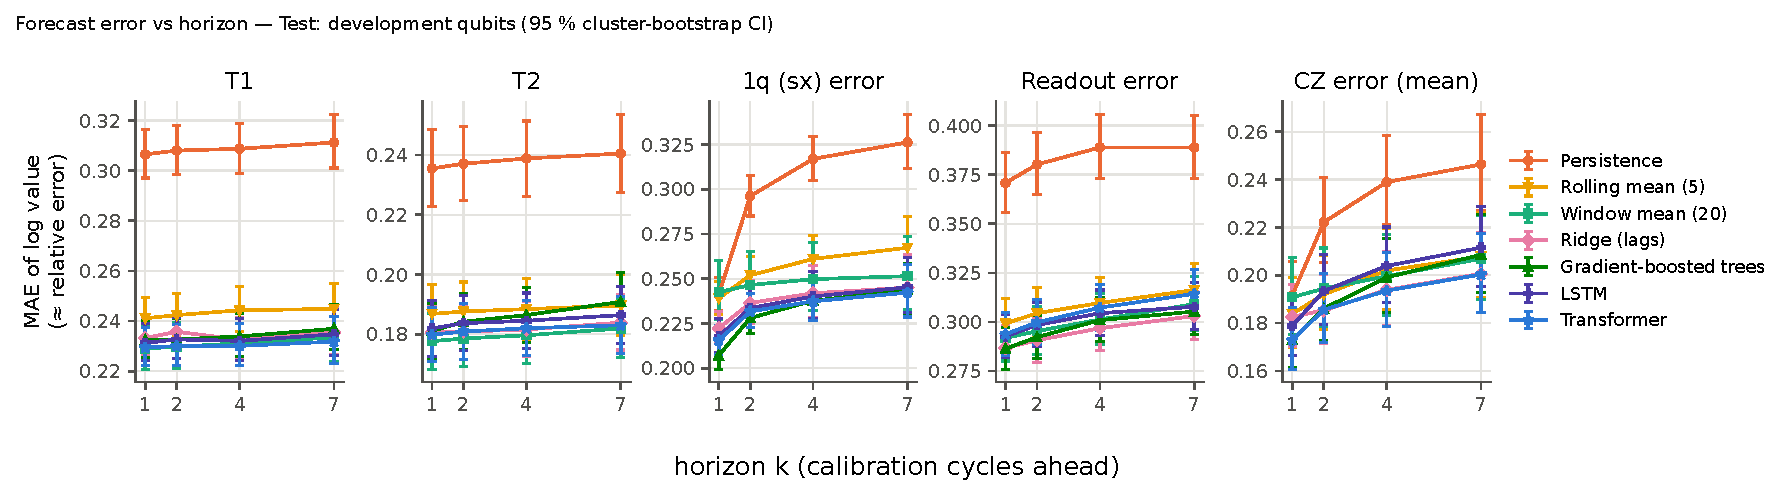
\includegraphics[width=0.98\linewidth]{mae_vs_horizon_test_primary.pdf}
\begin{itemize}\small
\item \textbf{How to read:} lower is better; each panel is one calibration property; bars are 95\% confidence intervals.
\item Persistence (orange) is clearly worst. All other models cluster together, and the Transformer (blue) is \textbf{not separated} from the window mean, ridge or trees.
\end{itemize}
\end{frame}

% =========================================================== B3
\begin{frame}{Result 1 (cont.): why averaging works so well}
\begin{columns}[c]
\column{0.55\textwidth}
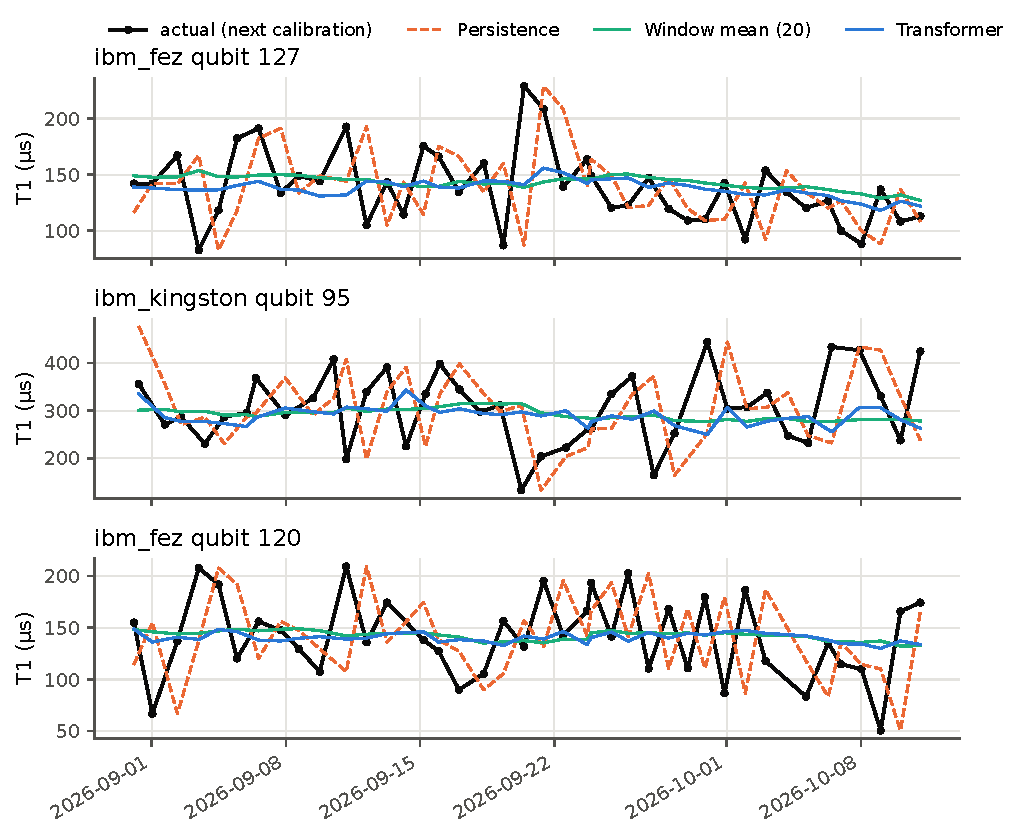
\includegraphics[width=\linewidth]{examples_log_t1_k1_test_primary.pdf}
\column{0.45\textwidth}
\begin{itemize}\small
\item Black: actual next-calibration $T_1$ of three test qubits. Dashed orange: persistence. Blue: Transformer.
\item $T_1$ jumps up and down by tens of \textmu s from day to day; 51\% of next-calibration values change by more than 25\%.
\item Persistence chases this noise; the models predict the slowly moving level, which is where most of their accuracy comes from.
\end{itemize}
\end{columns}
\end{frame}

% =========================================================== B4
\begin{frame}{Result 1 (cont.): generalisation to unseen qubits and device}
\centering
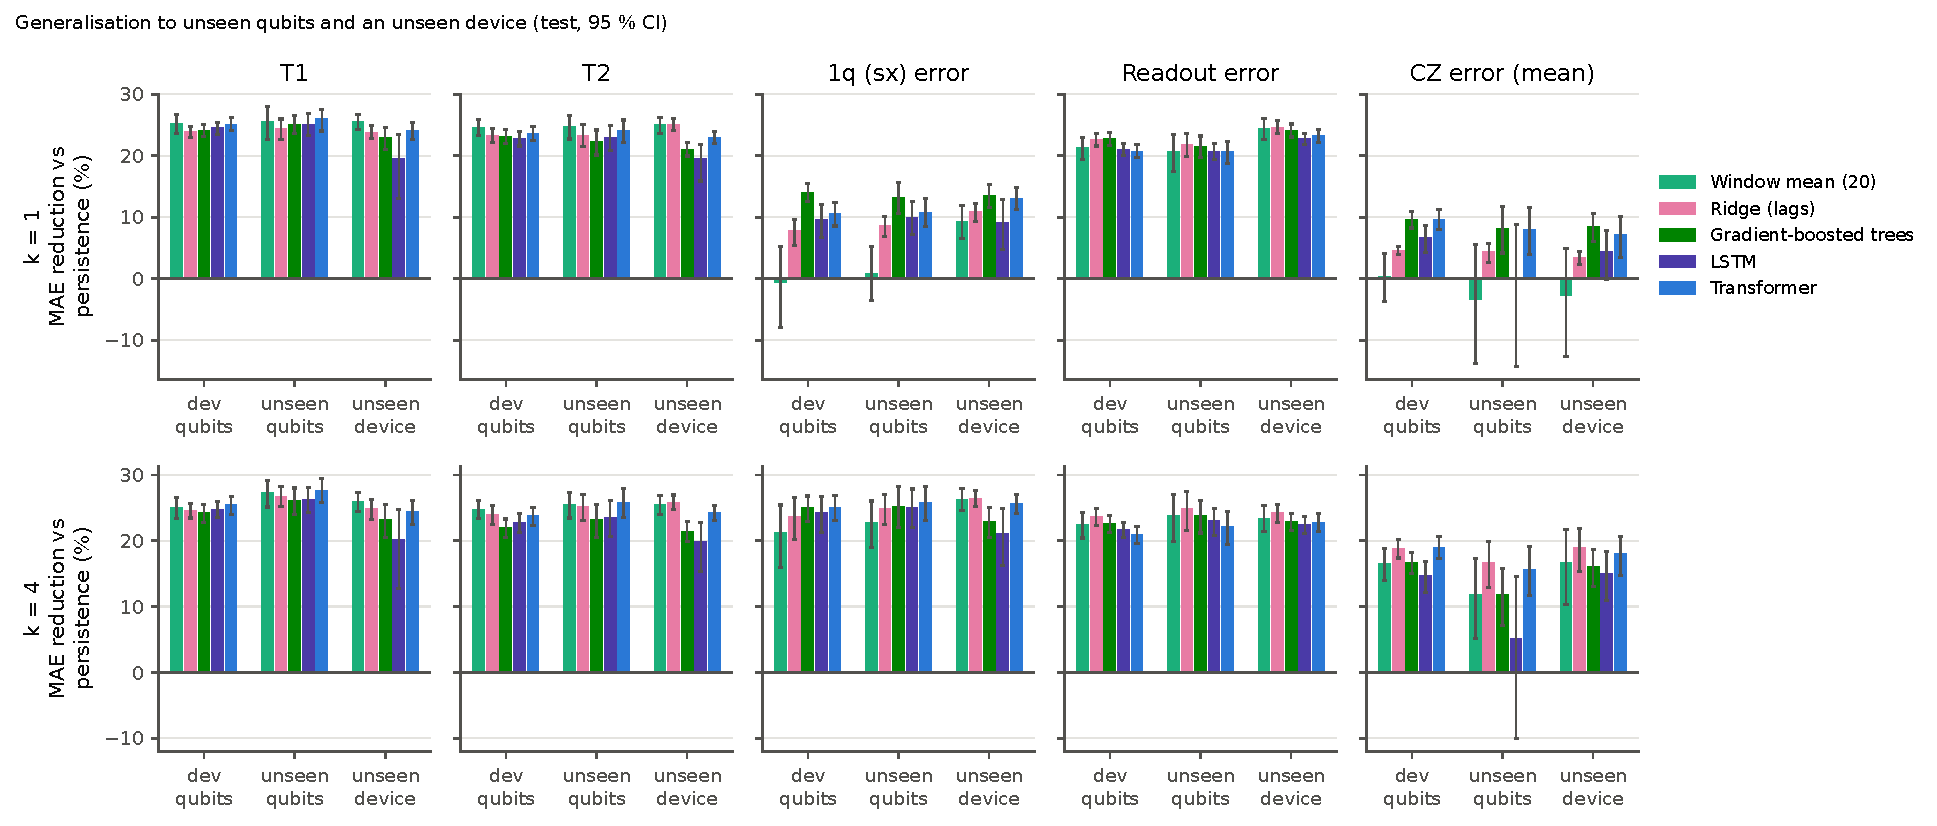
\includegraphics[width=0.82\linewidth]{generalisation_test.pdf}
\begin{itemize}\small
\item Models trained on ibm\_fez and ibm\_kingston transfer \textbf{without retraining} to unseen qubits and to the unseen ibm\_marrakesh.
\item The ranking among the top models is unstable: on the unseen device ridge and the window mean edge out the Transformer.
\end{itemize}
\end{frame}

% =========================================================== B5
\begin{frame}{Pair-level CZ forecasting (the quantity that drives decisions)}
\begin{columns}[c]
\column{0.6\textwidth}
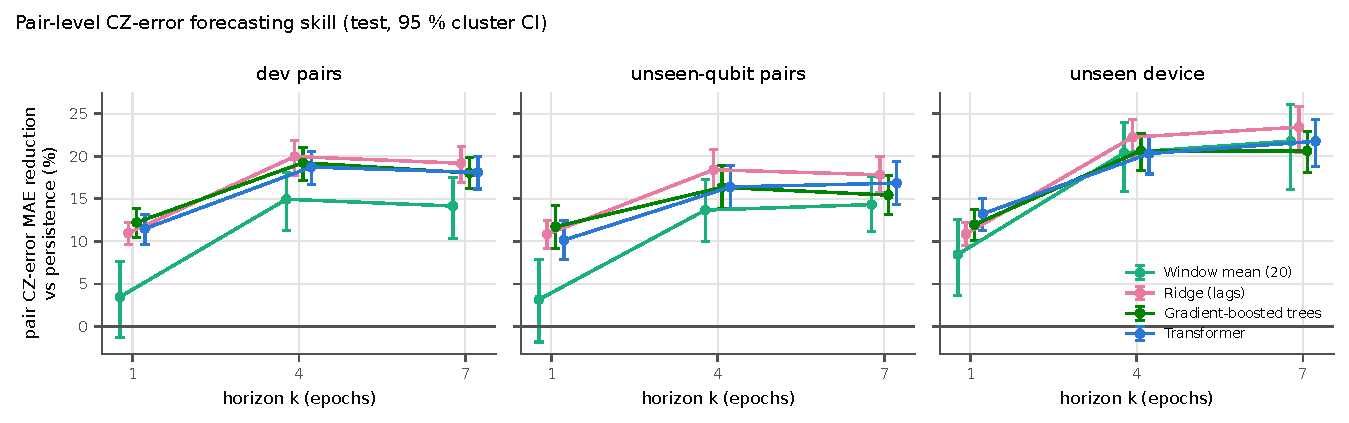
\includegraphics[width=\linewidth]{pair_forecast_skill_test.pdf}
\column{0.4\textwidth}
\begin{itemize}\small
\item Circuit error is dominated by two-qubit (CZ) errors, so we also forecast the CZ error of each coupled pair, 1, 4 and 7 \textbf{days} ahead (daily chip-wide epochs; a separate task from per-qubit forecasting).
\item Learned forecasters beat persistence by \good{11--12\%} (1 day) and \good{18--20\%} (4--7 days).
\item The Transformer is again level with ridge and gradient-boosted trees.
\end{itemize}
\end{columns}
\end{frame}

% =========================================================== B6
\begin{frame}{Evaluation protocol and hypotheses}
\begin{columns}[T]
\column{0.52\textwidth}
\textbf{Pre-registered hypotheses}
\begin{itemize}
\item \textbf{H1}: Transformer forecasts better than every baseline
\item \textbf{H2} (primary): Transformer-driven adaptation beats persistence, 1 day ahead
\item \textbf{H3}: beats the best fixed action; not worse under stationary noise
\item \textbf{H4}: beats the contextual bandit
\end{itemize}
\column{0.45\textwidth}
\textbf{Statistics}
\begin{itemize}
\item Error = mean over observables of $\mathbb{E}\,|\hat{E}-E_{\mathrm{ideal}}|$
\item Paired differences, 95\% cluster bootstrap over qubit chains
\item Holm correction for multiple tests
\item Test period evaluated once after freezing input hashes
\end{itemize}
\end{columns}
\end{frame}

% =========================================================== B7
\begin{frame}{Result 2 (cont.): paired comparison plot}
\begin{columns}[c]
\column{0.58\textwidth}
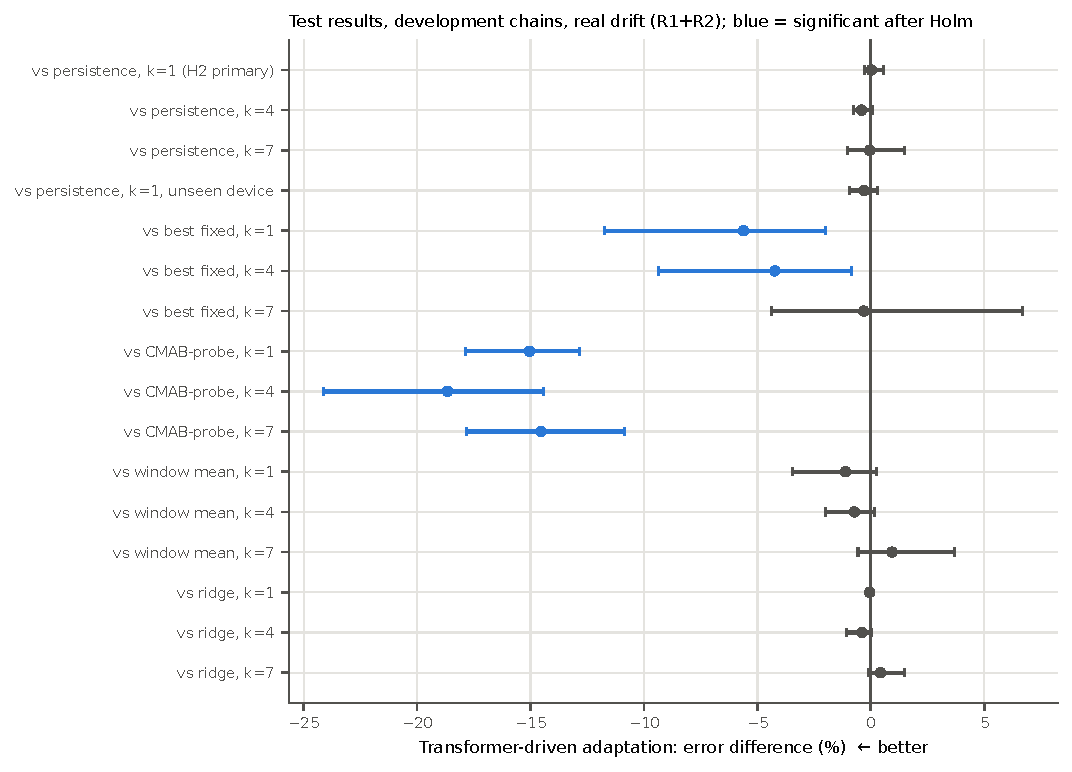
\includegraphics[width=\linewidth]{hypotheses_test.pdf}
\column{0.42\textwidth}
\begin{itemize}\small
\item Each row: error of Transformer-driven adaptation minus an alternative, in \%. Left of zero = Transformer better.
\item \textbf{Blue} rows are significant after Holm correction.
\item All rows against persistence, window mean and ridge sit on zero.
\item Large, significant gains only against the \textbf{best fixed} action and the \textbf{bandit}.
\end{itemize}
\end{columns}
\end{frame}

% =========================================================== B8
\begin{frame}{Result 3: error by decision horizon}
\begin{columns}[c]
\column{0.58\textwidth}
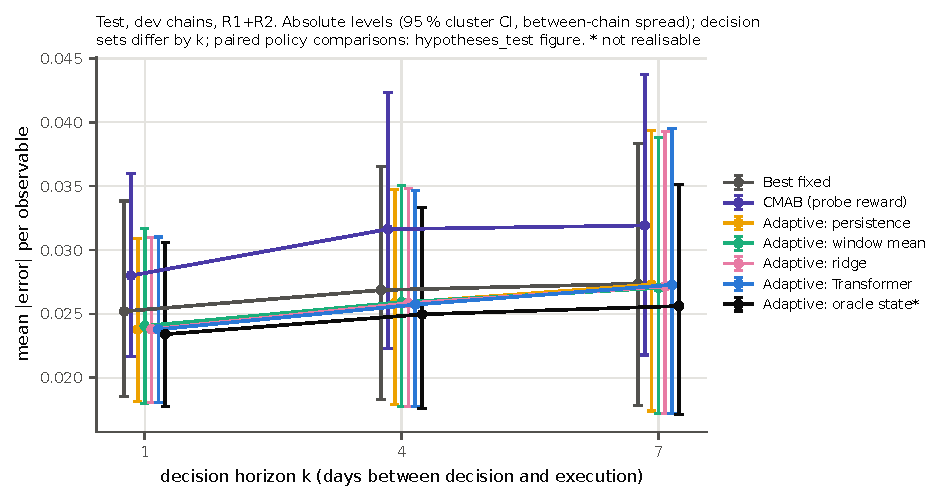
\includegraphics[width=\linewidth]{error_by_horizon_test.pdf}
\column{0.42\textwidth}
\begin{table}\scriptsize
\begin{tabular}{lccc}
\toprule
 & 1 d & 4 d & 7 d \\
\midrule
Best fixed & .0246 & .0263 & .0267 \\
Bandit & .0277 & .0309 & .0316 \\
Persistence & .0239 & .0259 & .0272 \\
Transformer & .0239 & .0258 & .0270 \\
Oracle & .0235 & .0251 & .0258 \\
\bottomrule
\end{tabular}
\end{table}
{\scriptsize Mean error per observable, incoherent regime (R1) only, development chains. Hypothesis tests pool R1 and R2.}
\begin{itemize}\scriptsize
\item Error grows with horizon; the bandit is highest everywhere.
\item The gap between persistence and the oracle widens with horizon, but the Transformer does not close it.
\end{itemize}
\end{columns}
\end{frame}

% =========================================================== B9
\begin{frame}{Value of information across policies (validation)}
\begin{columns}[c]
\column{0.6\textwidth}
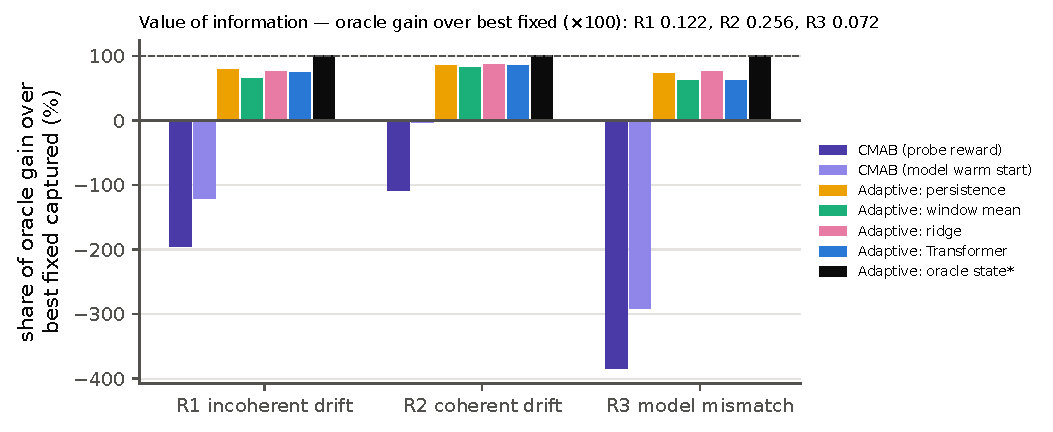
\includegraphics[width=\linewidth]{value_of_information.pdf}
\column{0.4\textwidth}
\begin{itemize}\small
\item Share of the oracle's gain over the best fixed action that each policy captures (100\% = as good as the oracle).
\item Calibration-informed controllers capture \good{61--87\%} (45--87\% when rerun after the epoch-timing fix), whichever state estimate they use.
\item The bandit variants are \bad{below zero}: worse than the best fixed action.
\end{itemize}
\end{columns}
\end{frame}

\end{document}
